\chapter{Sending OSC to Stellar Command} \label{chap:launchosc}
There are primarily two ways to use Stellar Command. The first is as a separate process that runs on the compute. The second method is to use Stellar Command as a library that you link to directly in your program. If you intend to use Stellar Command as a library, you can skip forward to chapter~\ref{chap:libraryosc} --
\emph{\titleref{chap:libraryosc}}. 

This chapter defines sending OSC to Stellar Command.  Examples for using OSC can be found at 
chapter~\ref{chap:oscexamples} --
\emph{\titleref{chap:oscexamples}}


\section{Launching Stellar Command} \label{sec:launchcommand}
%makeidx{standalone}
\index{OSC Configuration!Commandline arguments}
\index{OSC Configuration! Client port}
Scripts are provided to save you having to type these parameters each time and is described in section ~\ref{sec:configscript} --
\emph{\titleref{sec:configscript}}. This section, however, will explain in detail what each parameter does.
The Stellar Command module is instantiated by executing Java  with the name of the JAR file and the required program arguments that define communication, such as the network port to send OSC messages to, and the OSC address space.  
For example, to start the StellarCommand module so it sends OSC messages on UDP port 1234  using an OSC address space of \texttt{/Stellar},\footnote{In this instance, the OSC client and stellarium are on the same computer.} one would execute the following command:\\

\begin{syntax} \index{Commandline arguments!port} \index{Commandline arguments!osc}
\medskip
	java -jar StellarCommand.jar port=1234 osc=/Stellar  \\
\medskip
\end{syntax}
\bigskip
   When the server starts, it will open the first available UDP port, and notify the client of this port. For example, if the command module opened port 4567, it will send an OSC message \texttt{/Stellar/osc 4567} to the client on the localhost. 
   
\begin{syntax}
\medskip
	/Stellar/osc 4567  \\
\medskip
\end{syntax}
\bigskip

\index{OSC Configuration!Stellar Command receive port} \index{Commandline arguments!tryport}
Allowing the command module to find its own port number removes the probability of port clashes as each client furnishes the other with a valid port number for communicating without requiring configuration in the command module. It is, however, possible to request the Stellar Command module try certain ports by adding the argument \textit{tryport} with a comma separated list of ports. For example, the argument \texttt{tryport=3333,4444,5555} will cause stellarium to sequentially try opening the ports listed, and if these all fail, will then open the first available port.\\
   
   \begin{syntax}
\medskip
   	java -jar StellarCommand.jar port=1234 osc=/Stellar  tryport=3333,4444,5555\\
\medskip
   \end{syntax}
   \bigskip
   
   The OSC client would receive the following OSC message:
   \begin{syntax}
   	/Stellar/osc 3333  \\
   \end{syntax}
   \bigskip
   
The OSC client and the stellarium server do not have to be on the same physical computer as the Stellar Command module. For example Figure~\ref{fig:RemoteStellarium}, shows three OSC clients and a stellarium server on a LAN, and a remote stellarium server accessible from the internet through \textit{myserver.com}.

\begin{figure}[htbp]
	\centering
	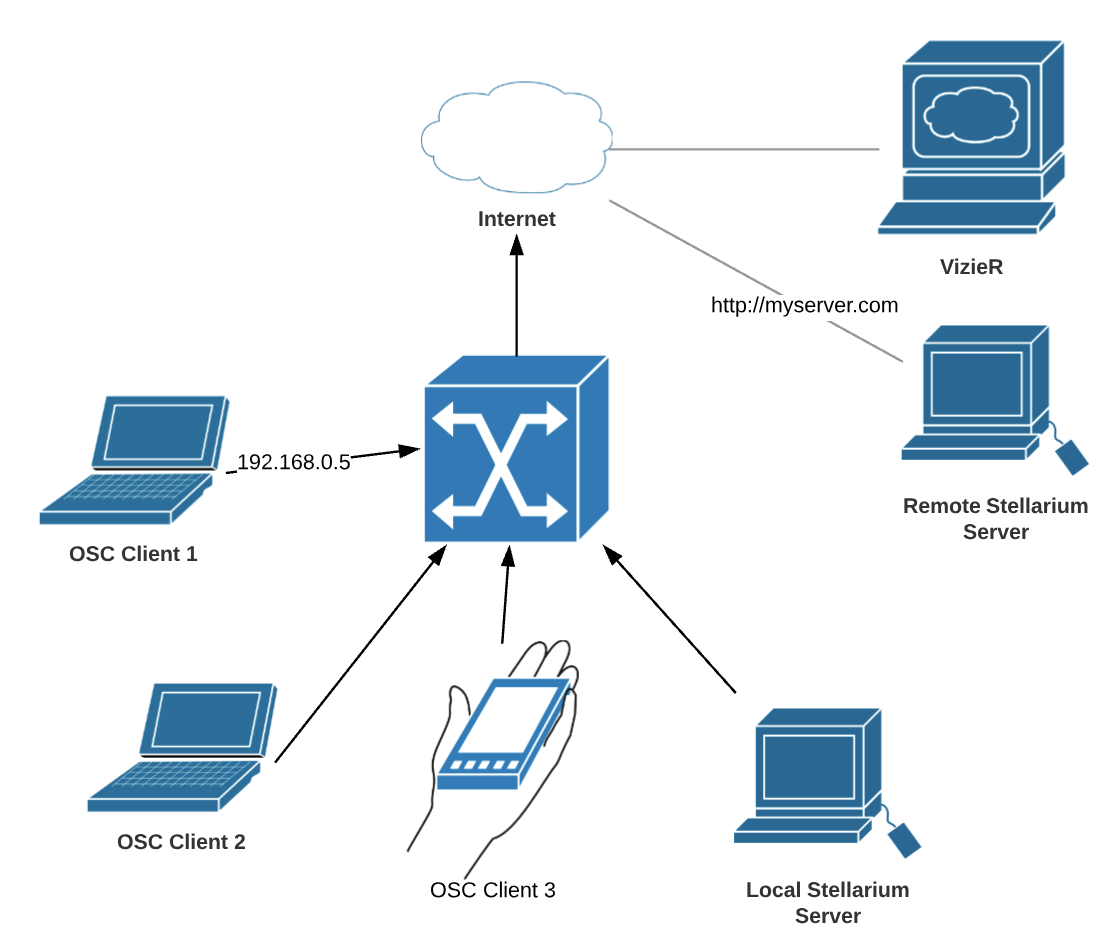
\includegraphics[width=1\columnwidth]{RemoteStellarium}
	\caption{Remote Stellarium and OSC Clients.}
	\label{fig:RemoteStellarium}
\end{figure}
\bigskip

Creating a connection between \textit{OSC Client 1} and \texttt{Remote Stellarium Server} is effected by adding adding the arguments \\\texttt{client=192.168.0.5} and \texttt{stellarium=http://myserver.com} to the command line.
This will cause the Stellar Command module to send OSC messages to ``192.168.0.5" and stellarium commands to \textit{http://myserver.com} on HTP port 8090\footnote{The default stellarium Remote Control port is 8090, however, this can be changed inside stellarium. It is assumed that port forwarding when not using a local area network has been configured to send packages to the correct computer hosting Stellarium}, effectively acting as a proxy between the two.

 \begin{syntax} \index{Commandline arguments!client}\index{Commandline arguments!stellarium}
	\medskip
	java -jar StellarCommand.jar port=1234 osc=/Stellar  {\char'134}\\client=192.168.0.5 stellarium=http://myserver.com\\
	\medskip
\end{syntax}
\bigskip

\index{Commandline arguments!client}\index{Commandline arguments!Stellarium poll frequency} \index{Commandline arguments!stellariumpoll}
Stellar Command works by polling Stellarium to detect changes. This is a requirement because Stellarium uses a REST API rather than a persistent socket. By default, the Stellarium will be polled once per second, however, you can change this by adding a parameter \textit{stellariumpoll}, which dictates how often Stellarium is polled in milliseconds. For example, the following would cause Stellarium to be polled approximately  every two seconds. Although the parameter is in milliseconds, causing Stellarium to poll more often than once per second can slow your system down significantly. 

 \begin{syntax} 
	\medskip
	java -jar StellarCommand.jar port=1234 osc=/Stellar  {\char'134}\\stellariumpoll=2000 
	\medskip
\end{syntax}
\bigskip
If you set a polling time of zero, then Stellarium will not be polled, however, you can request a poll from your own application be sending the \textit{poll} command - described in section \refsection{sec:poll}.


\index{Commandline arguments!client}\index{Commandline arguments!Stellarium remote port}\index{Commandline arguments!stellariumport}
The default Stellarium Remote Control port is 8090, however, this can be changed inside Stellarium. It is assumed that port forwarding when not using a local area network has been configured to send packages to the correct computer hosting Stellarium. You can configure this in Stellar Command by adding the parameter \textit{stellariumport}, which dictates the port Stellar Command will use to attempt to communicate with Stellarium. For example, the following would cause Stellar Command to communicate with Stellarium on port 2000. It is extremely unlikely you would need to change this parameter, however, the facility is there in case you do need to.   

\begin{syntax} 
	\medskip
	java -jar StellarCommand.jar port=1234 osc=/Stellar  {\char'134}\\stellariumport=2000 
	\medskip
\end{syntax}
\bigskip

\subsection{Launch Without Stellarium}\label{sec:launchnostellarium}\index{OSC messages to Stellar Command!Running without Stellarium}. In some cases, you may want to launch Stellar Command to access the functionality of VizieR without using Stellarium. This may be the case if you are only interested in the astronomical data and are not using Stellarium as an interface device. This  is be accomplished by adding the value \textit{disabled} to the \textit{stellarium} parameter. For example, the following command line argument will disable calls to Stellarium.

 \begin{syntax} \index{Commandline arguments!client}\index{Commandline arguments!stellarium} \index{Commandline arguments! disable Stellarium}
	\medskip
	java -jar StellarCommand.jar port=1234 osc=/Stellar  {\char'134} stellarium=disabled\\
	\medskip
\end{syntax}
\bigskip



\subsection{Using Configuration Scripts}\label{sec:configscript}
\index{OSC Configuration!Using a script}
Three scripts are provided to facilitate simple configuration and launching of  Stellar Command. The script \textit{runStellarCommand.sh} is used to configure and launch Stellar Command from the commandline in MacOS and Linux. \index{OSC Configuration!MacOS Commandline}  \index{OSC Configuration!Linux Commandline} The file \textit{runStellarCommand.bat} is used to configure and launch on Windows  \index{OSC Configuration!Windows batch file}. There is an additional file, \textit{runStellarCommand.command}, which allows a person to write the configuration inside the \textit{.sh} file and then launch Stellar Command by double clicking \textit{runStellarCommand.command} with the mouse.

Configuring Stellar Command is done simply by replacing the value in the script with those required.
 \begin{syntax} \index{Commandline arguments!client}\index{Commandline arguments!stellarium}
	\medskip
PORT=1234\\
OSC=/Stellar\\
TRYPORTS="3333,4444,5555"\\
CLIENT=\\
STELLARIUM=\\ 
STELLARIUMPOLL=\\
STELLARIUMPORT=\\
	\medskip
\end{syntax}
\bigskip

If, for example, you wanted Stellar Command to send it's messages to your client on port 5678, simply change text after  \textit{PORT=}.
 \begin{syntax} \index{Commandline arguments!client}\index{Commandline arguments!stellarium}
	\medskip
	PORT=5678\\
	\medskip
\end{syntax}
\bigskip

The same applies for the other parameters.

\section{Sending Commands to the Stellar Command Module}
You can provide instructions to Stellar Command in order to control stellarium or to change the amount and type of data you want to receive. For example, you may want the stellarium display to zoom in closer to a particular area of sky. You would do this by decreasing the field of view.\footnote{Section~\ref{subsec:fieldofview} --
	\emph{\titleref{subsec:fieldofview}} shows how to do this.} Likewise, you may want to reduce the amount of astronomical data you are receiving by adding a filter threshold so VizieR will only receive stars within a certain magnitude range. 

Message names are not case sensitive. For example, the messages \textit{fieldOfView} and \textit{FieldOfView} could both be used to set the field of view for stellarium.

\subsection{poll}  \label{sec:poll} \index{OSC messages to Stellar Command!poll}  \index{OSC messages to Stellar Command!Request Version}
Sometimes Stellar Command may already be started and configured to send and listen to the ports. You can easily find this out by sending the \textit{poll} command with no arguments, which will cause Stellarium to reply on the ports it is configured when started up. Additionally, the poll message will cause Stellar Command to return the running version of Stellar Command.

 \begin{syntax}
	\medskip
	Stellar/poll
	\medskip
\end{syntax}

If you were sending OSC on the required port and your client was at the correct address, you would receive the following OSC message:
\begin{syntax}
	/Stellar/osc 3333  \\
\end{syntax}
\bigskip

See sections \refsection{sec:version} and \refsection{sec:osc}for more detail.

\subsection{queryVizieR}\label{subsec:queryVizieR}  \index{OSC messages to Stellar Command!queryVizieR}\index{OSC messages to Stellar Command!Direct VizieR Query}\index{OSC messages to Stellar Command!Running without Stellarium}
It is possible to run Stellar Command and make calls to  VizieR without running Stellarium, as detailed in section \refsection{sec:launchnostellarium}. This might be the case if you were only interested in the astronomical data without any correlation to  a Stellarium Display, for example, if you were using a graphic programs such as Processing. The call is made by defining a centre radius as a float. If querying using RA and Dec, the second and third arguments are floats. For example, the following call would query a 1\degree  radius at an RaDec of  186.6492, -63.0989

\begin{syntax} \index{VizieR query!Ra and Dec}
	/Stellar/osc 1.0 186.6492 -63.0989  \\
\end{syntax}
\bigskip
 
 Additionally, it is possible to query using a star or celestial object instead of RA and Dec. For example, to query a 1\degree circle around Acrux would be performed as follows:
  
 \begin{syntax} \index{VizieR query!Ra and Dec}
 	/Stellar/osc 1.0 Acrux  \\
 \end{syntax}
 \bigskip

Stellar Command will respond by sending Star Values as OSC messages. See section \refsection{sec:version} for details on Star Values.

\subsection{fieldOfView}\label{subsec:fieldofview}\index{OSC messages to Stellar Command!fieldOfView}

In order to send a change in the field of view, send a message using the \textit{fieldOfView} in the namespace, followed by the field of view as a float argument. For example, to set the field of view to 60$^{\circ}$, you would send a message as follows:
 \begin{syntax}	
 	\medskip
	/Stellar/fieldOfView 60.0
	\medskip
 \end{syntax}
\bigskip

 \subsection{time} \index{OSC messages to Stellar Command!time}
You can set the simulation time by sending a full ISO time stamp as a string message, or by sending each Date time parameter as OSC arguments. For example, you can set the time as a string as follows:

\begin{syntax}	
	\medskip
	/Stellar/time 2019-04-18T17:51:17Z
	\medskip
\end{syntax}

If using specified time, the first three arguments will be  Year, Month and  Day as integers. The next  argument will be the hour as an integer as a 24 hour number. EG, the number 13 will signify 1pm. The next two arguments will be the minutes and seconds as integers.  The final optional argument will be the time zone, using Z for zero time, or -/-HH:MM for a different GMT time shift.

The following will set to 5:51:17pm on 18 April 2019 at GMT.

\begin{syntax}	
	\medskip
	/Stellar/time 2019 4 18 17 51 17 Z
	\medskip
\end{syntax}

The following will set to 5:51:17pm on 18 April 2019 at GMT + 5 Hours. Note that you must add the "+" or "-" sign and it must be a string value. 
\begin{syntax}	
	\medskip
	/Stellar/time 2019 4 18 17 51 17 +05:00
	\medskip
\end{syntax}

If the time zone is blank, the local time at the location will be used. 
Sending the following would set to midday on 18 April 2019 at the Observer location in Stellarium.

\begin{syntax}	
	\medskip
	/Stellar/time 2019 4 18 12 0 0 
	\medskip
\end{syntax}

You can also set the time by typing the exact string value.
\begin{syntax}	
	\medskip
	/Stellar/time 2019-04-06T12:00:00Z 
	\medskip
\end{syntax}


\subsection{moveLR} \index{OSC messages to Stellar Command!moveLR}
You can make the stellarium display move left or right by sending the command \textit{moveLR} followed by a floating point number indicating how far to move. A positive value will make it appear that the viewer is turning their head to the right, while a negative number will simulate moving to the left. To move to the right, send the following command:
  \begin{syntax}	
 	\medskip
 	/Stellar/moveLR 1.0
 	\medskip
 \end{syntax}
 \bigskip

\subsection{moveUD} \index{OSC messages to Stellar Command!moveUD}
You can make the stellarium display move up or rdown by sending the command \textit{moveUD} followed by a floating point number indicating how far to move. A positive value will make it appear that the viewer is turning their head up, while a negative number will look lower. To look towards the sky, send the following command:
\begin{syntax}	
	\medskip
	/Stellar/moveUD 1.0
	\medskip
\end{syntax}
\bigskip

\subsection{azimuth} \index{OSC messages to Stellar Command!azimuth} \label{subsec:azimuth}
If you want to change the azimuth that you are looking at, use \textit{azimuth} in the namespace and add the azimuth as a float argument. For example, if you wanted to turn to the east, you would send a message as follows:
 \begin{syntax}	
	\medskip
	/Stellar/azimuth 90.0
	\medskip
\end{syntax}

\subsection{altitude} \index{OSC messages to Stellar Command!altitude}
If you want to change the altitude that you are looking at, use \textit{altitude} in the namespace and add the altitude as a float argument. For example, if you wanted to look 45$^{\circ}$ up, you would send a message as follows:
\begin{syntax}	
	\medskip
	/Stellar/altitude 45.0
	\medskip
\end{syntax}

\subsection{viewAltAz} \index{OSC messages to Stellar Command!viewAltAz}
Setting the altitude and the azimuth at the same time is so commonplace that it has been made available as a single OSC message.
If you want to change the altitude that you are looking at, use \textit{viewAltAz} in the namespace and add the altitude and then the azimuth as float arguments. The two previous calls could have been done with the single command
\begin{syntax}	
	\medskip
	/Stellar/viewAltAz 45.0 90.0
	\medskip
\end{syntax}

\subsection{viewRADec} \index{OSC messages to Stellar Command!viewRADec}
You can move to the RA and Dec to the centre of the sky by using  \textit{viewRADec} in the namespace and send the RA and Dec as decimal degrees. If for example, you wanted to centralise  an RA of 95.98796$^{\circ}$  and Dec. of -52.69566$^{\circ}$  (this is the star Canopus), you would send the following OSC:
 \begin{syntax}	
 	\medskip
 	/Stellar/viewRADec 95.98796 -52.69566
 	\medskip
 \end{syntax}
 
 \subsection{viewObject}  \index{OSC messages to Stellar Command!viewObject}
 You may want to select a particular named object in the sky, such as a star, planet or moon. You can do this by using the command \textit{viewObject} followed by the object name. For example, if you wanted to centre the planet Saturn, you would send the following OSC:
 
\begin{syntax}	
 	\medskip
 	 /Stellar/viewObject Saturn
 	\medskip
 \end{syntax}
 
 \subsection{viewerObservationPoint} \index{OSC messages to Stellar Command!viewerObservationPoint}
 You can change the latitude, longitude, altitude and planet you are setting as your observation point by using the \textit{viewerObservationPoint} command followed by the latitude, longitude, and altitude as float arguments, and the planet as a string.  For example, to set a latitude of 32$^{\circ}$, longitude of 151$^{\circ}$, and altitude of 21m from Saturn, you would send the following command:
 
 \begin{syntax}	
 	\medskip
 	/Stellar/viewerObservationPoint 32.0 151.0 21.0 Saturn
 	\medskip
 \end{syntax}
 
 
 \subsection{showGround }\index{OSC messages to Stellar Command!showGround}
 It is possible to hide the ground, enabling you to see stars and planets through the earth by sending the \textit{showGround } command, and an integer value of zero to hide the ground or non-zero to show it. To hide the ground, you would send the following OSC message:
 
  \begin{syntax}	
 	\medskip
 	/Stellar/showGround 0
 	\medskip
 \end{syntax}

 \subsection{showAtmosphere}\index{OSC messages to Stellar Command!showAtmosphere}
It is possible to hide the atmosphere, enabling you to see stars and planets during daylight hours by sending the \textit{showAtmosphere} command, and an integer value of zero to hide the atmosphere or non-zero to show it. To hide the atmosphere, you would send the following OSC message:

\begin{syntax}	
	\medskip
	/Stellar/showAtmosphere 0
	\medskip
\end{syntax}

 \subsection{showStarLabels}\index{OSC messages to Stellar Command!showStarLabels}
It is possible to hide the star labels  by sending the \textit{showStarLabels} command, and an integer value of zero to hide the labels or non-zero to show it. To hide the labels, you would send the following OSC message:

\begin{syntax}	
	\medskip
	/Stellar/showStarLabels 0
	\medskip
\end{syntax}

 \subsection{showConstellationart}\index{OSC messages to Stellar Command!showConstellationArt}
It is possible to show or hide the constellation art by sending the \textit{showConstellationart} command, and an integer value of zero to hide the art or non-zero to show it. To show the constellation art, you would send the following OSC message:

\begin{syntax}	
	\medskip
	/Stellar/showConstellationart 1
	\medskip
\end{syntax}

\subsection{timeRate}\index{OSC messages to Stellar Command!timeRate}\index{TimeRate!Sending OSC} 
It is possible to change the simulated time rate on Stellarium by sending the \textit{timeRate} command followed by the new time rateas a float. If, for example, you set the time rate to zero, time would be still and the stars would not move through the sky. If, however, you set the time rate to 2.0, the display would simulate time running at twice normal speed. You can also make time go in reverse by setting the time rate to a negative number. To set the display to simulate time running at twice normal speed, you would send the following:

\begin{syntax}	
	\medskip
	/Stellar/timeRate 2.0
	\medskip
\end{syntax}

See section ~\ref{subsec:timerate} --
\emph{\titleref{subsec:timerate}} for time rate specifics.

\subsection{saveTable and loadTable} \index{OSC messages to Stellar Command!saveTable}  \index{OSC messages to Stellar Command!loadTable}
Retrieving astronomical data from VizieR can sometimes take time, depending on your internet speed and the number of stars in the field of view requested. It is possible to save the current loaded VizieR table of stars to a file so you can use it even when there is no internet. To save the table, send the command \textit{saveTable} followed by the name of the file you want it saved to. You can then use the \textit{loadTable} command later to load the data and have Stellar Command send it to you.
To save the current table to the file "Acrux.txt", send the following command:
 
 \begin{syntax}	
 	\medskip
 	/Stellar/saveTable Acrux.txt
 	\medskip
 \end{syntax}

To load this table from file and have it send the data to you, send the following command:
 \begin{syntax}	
	\medskip
	/Stellar/loadTable Acrux.txt
	\medskip
\end{syntax}

\subsection{sendStars} \index{OSC messages to Stellar Command!sendStars}
It is possible to pause Stellar Command sending stars data back to the client. This may be particularly useful if you are receiving data from thousands of stars and the resources to parse decode all that data in OSC may be unnecessary. Sending the \textit{sendStars} command with a zero will cause Stellar Command to stop querying VizieR, and thus stop sending you updated astronomical data. You will still, however, receive position and field of view change messages. Sending a non-zero argument with the command will resume sending starts. To stop the data being sent, send OSC as follows:

 \begin{syntax}	
	\medskip
	/Stellar/sendStars 0
	\medskip
\end{syntax}  

\subsection{filter}  \index{OSC messages to Stellar Command!filter} \index{Filters!Hpmag}
Considering how many stars could be within a particular view, it can be beneficial to apply a filter.  For example, you may only be interested in stars with a magnitude brighter that 6. Setting a filter actually modifies the query sent to VizieR, thus reducing the amount of time to process the astronomical data.
Filtering the data is accomplished by adding the command \textit{filter}, followed by the astronomical data filed you want to filter, followed by less or greater and then using the OSC argument as the filter value.  for example, to filter the \textit{Hpmag} field so magnitudes brighter (less than) 6.5 are returned, you would send the following OSC command
   
    \begin{syntax}	 \index{OSC messages to Stellar Command!filter/Hpmag/less}  
   	\medskip
   	/Stellar/filter/Hpmag/less 6.5
   	\medskip
   \end{syntax}  

You can AND filters together by sending a second command. for example, to filter stars that are between magnitudes 3 and 6, you would send the following OSC.
    \begin{syntax}	 \index{OSC messages to Stellar Command!filter/Hpmag/greater}
	\medskip
	/Stellar/filter/Hpmag/less 6\\
	/Stellar/filter/Hpmag/greater 3
	\medskip
\end{syntax}  

You can filter by star colour (i.e. temperature) by filtering \textit{B-V}. For example, to filter stars with  B-V values between -1 and 1, you apply the following OSC commands:  \index{Filters!B-V}
     \begin{syntax}	 \index{OSC messages to Stellar Command!filter/B-V/less}  \index{OSC messages to Stellar Command!filter/B-V/greater}
 	\medskip
 	/Stellar/filter/B-V/less 1\\
 	/Stellar/filter/B-V/greater -1
 	\medskip
\end{syntax}  

You can reset the specific filter by sending a \textit{reset} command with the filter. Eg, to cleat the Hpmag filters, send the following OSC:  \index{OSC messages to Stellar Command!filter/Hpmag/reset}
    \begin{syntax}	
	\medskip
	/Stellar/filter/Hpmag/reset
	\medskip
\end{syntax}  
	\medskip

You can reset all filters by sending the \textit{resetFilters} command: \index{Filters!reset}
	\medskip
\begin{syntax}	
	\medskip
	/Stellar/resetFilters
	\medskip
\end{syntax}  
	\medskip
\subsection{script}\label{sec:scriptcommand} \index{OSC messages to Stellar Command!script} \index{Stellarium Script!Start}
An extremely powerful feature of Stellarium is the ability to run predefined astronomy shows. These scripts are written in JavaScript and are run within the Stellarium core. You can run, stop or find out the status of the scripting engine in Stellarium with the \textit{script command}.

You can run a specific script by setting the first OSC argument as the name of the script. Sending the following OSC message would cause the \textit{The Jack Bennett Catalog} packaged with Stellarium to run.
\begin{syntax}	
	\medskip
	/Stellar/script bennett.ssc
	\medskip
\end{syntax}  
	\medskip
	
If you choose to keep your scripts separate to those packaged with Stellarium, you will need o pass the full path as the OSC argument. For example, 
	\medskip
\begin{syntax}	
	\medskip
	/Stellar/script /Stellar/script /Users/me/myprivatescripts/stellariumscript/bennett.ssc
	\medskip
\end{syntax}  
	\medskip
Stopping a script is done by using the word "stop" as the OSC argument. 
	\medskip
\begin{syntax}	
	\medskip
	/Stellar/script stop
	\medskip
\end{syntax}  
	\medskip
Calling the script command without an argument will cause Stellar Command to send back the scripting engine status. Section \refsection{sec:scriptstatus} details the status of a returned script status message.